% !TEX root = main.tex
% !TeX program = txs:///arara

%%% we use arara because it makes life easier
%%% arara should work on all platforms
% arara: lualatex: { draft: true, shell: true}
% arara: xindy: {modules: [texindy, page-ranges], codepage: utf8, language: german-duden}
% !arara: --> if changed('idx')
% arara: biber if missing('bbl') || found('log', 'Citation')
% arara: --> || found ('log', 'Please \\(re\\)run Biber')
% arara: makeglossaries if missing('gls') || changed('glo')
% arara: lualatex: { shell: true, synctex: true }
% arara: --> if found('log', 'No file ') || found('log', 'undefined references') || found('log', 'Rerun required') || found('log', 'Rerun to get cross-references')
% arara: lualatex: { shell: true, synctex: true }

%%% we source our input files to get a cleaner main.tex
%%% general page related settings
\documentclass[12pt,%
  %draft,%
  overfullrule=true,%
  oneside,%
  titlepage,%
  listof=totoc,%
  twoside=semi,%
  bibliography=totoc]{scrartcl} % https://www.ctan.org/pkg/scrartcl

\usepackage[automark,headsepline]{scrlayer-scrpage} % https://www.ctan.org/pkg/scrlayer-scrpage

\usepackage[a4paper,%
  left=3cm,%
  right=2.5cm,%
  top=2cm,%
  bottom=2cm]{geometry}

\usepackage{setspace} % 1,5 cm Zeilenabstand
\onehalfspacing{}

%\setlength{\parindent}{0mm} % https://komascript.de/faq_parindent
%\setlength{\parskip}{0.8em plus 0.5em minus 0.3em}
%\sloppy %Abstände variieren

%%% language settings
\usepackage{hyphsubst} % https://www.ctan.org/pkg/hyphsubst
\HyphSubstIfExists{ngerman-x-latest}{%
\HyphSubstLet{ngerman}{ngerman-x-latest}}{}
\usepackage[ngerman]{babel} % https://www.ctan.org/pkg/babel
\usepackage[babel,german=guillemets]{csquotes} % https://www.ctan.org/pkg/csquotes

%%% font settings
%\usepackage[utf8]{inputenc} % not needed with luatex
\usepackage{fontspec} % luatex needs this one
\setmainfont{Arial} % we even get to use Arial, woohoo..
\renewcommand\familydefault{\sfdefault} %defaults to helvetica
%%% if you don't or can't use luatex, use this
%% helvet is alternative to Arial for tex, or it's actually the original font
%% with minimal differences
%\usepackage[scaled=0.9]{helvet} % use together with courier package to avoid pixelated fonts
%\usepackage{courier}

% math related settings
\usepackage{amsmath} % https://www.ctan.org/pkg/amsmath
\usepackage{unicode-math} % https://www.ctan.org/pkg/unicode-math
\setmathfont{texgyrepagella-math.otf}
%\usepackage{mathptmx} % https://www.ctan.org/pkg/mathptmx -- obsolet
%\usepackage{nicefrac} % The pack­age type­sets fractions “nicely”
\usepackage{marvosym} % https://www.ctan.org/pkg/marvosym
\usepackage[hang, multiple]{footmisc} % must be placed above hyperref to avoid warnings
\setlength{\footnotemargin}{1em}
\usepackage[colorlinks=true,%
  breaklinks=true,%
  linkcolor=black,%
  citecolor=blue,%
  menucolor=black,%
  urlcolor=black]{hyperref} % adds new commands to include hyperlinks

%%% additional packages
\usepackage{ragged2e} % https://www.ctan.org/pkg/ragged2e
%\usepackage{footnote} % https://www.ctan.org/pkg/footnote
%\usepackage{fancybox} % https://www.ctan.org/pkg/fancybox

%%% table packages
\usepackage[table,xcdraw]{xcolor} % https://www.ctan.org/pkg/xcolor
\usepackage{multirow} % https://www.ctan.org/pkg/multirow
%\usepackage{array} % https://www.ctan.org/pkg/array
%\usepackage{colortbl} % https://www.ctan.org/pkg/colortbl
\usepackage{microtype} % https://www.ctan.org/pkg/microtype

%%% floats
\usepackage{float} % https://www.ctan.org/pkg/float
\usepackage{caption} % https://www.ctan.org/pkg/caption
\usepackage{graphicx} % https://www.ctan.org/pkg/graphicx

%%% list related
\usepackage{enumitem} % https://ctan.org/pkg/enumitem
%\usepackage{mdwlist} % https://www.ctan.org/pkg/mdwlist

%%% Glossary
\usepackage[%
  %sort=word,%
  xindy%
  ]{glossaries-extra} % https://www.ctan.org/pkg/glossaries
\setabbreviationstyle{long-short}
\loadglsentries{meta/gls.tex} % definitions go there
% index w/ xindy
\usepackage{makeidx} % https://www.ctan.org/pkg/makeidx
\usepackage{idxlayout} % https://www.ctan.org/pkg/idxlayout
\makeindex
%%% List of Abbreviations
\usepackage[refpage,refeq]{nomencl}
\makenomenclature

%%% Biblatex
\usepackage[%
  backend=biber,%
  style=numeric,%
  citestyle=authoryear,%
  %sortcase=true,%
  date=iso,%
  seconds=true,%
  urldate=iso,%
  %dashed=false,%
  %doi=false,%
  isbn=true,%
  %mergedate=false,%
  autocite=footnote,%
  sortlocale=de]{biblatex}
% Original Author: Andy Grunwald
% https://github.com/andygrunwald/FOM-LaTeX-Template/blob/master/skripte/weitereEbene.tex

% Optionen für Biblatex

% et al. an Stelle von u.a.
\DefineBibliographyStrings{ngerman}{%
   andothers = {{et\,al\adddot}},
}

% Klammern um das Jahr in der Fußnote
\renewbibmacro*{cite:labelyear+extrayear}{%
  \iffieldundef{labelyear}
    {}
    {\printtext[bibhyperref]{%
       \mkbibparens{%
         \printfield{labelyear}%
         \printfield{extrayear}}}}}

\DeclareNameFormat{last-first}{%
  \iffirstinits
    {\usebibmacro{name:family-given}
        {\namepartfamily}
        {\namepartgiveni}
        {\namepartprefix}
        {\namepartsuffix}
    }
    {\usebibmacro{name:family-given}
        {\namepartfamily}
        {\namepartgiven}
        {\namepartprefix}
        {\namepartsuffix}
    }%
  \usebibmacro{name:andothers}}

% Alternative Notation der Fußnoten
% Zeigt sowohl den Nachnamen als auch den Vornamen an
% Beispiel: \fullfootcite[Vgl. ][Seite 5]{Tanenbaum.2003}
\DeclareCiteCommand{\fullfootcite}[\mkbibfootnote]
  {\usebibmacro{prenote}}
  {\usebibmacro{citeindex}%
    \printnames[sortname][1-1]{author}%
    \addspace (\printfield{year})}
  {\addsemicolon\space}
  {\usebibmacro{postnote}}

%Autoren (Nachname, Vorname)
\DeclareNameAlias{default}{family-given}

%Reihenfolge von publisher, year, address verändern
% Achtung, bisher nur für den Typ @book definiert

%% Definiert @Book Eintrag
\DeclareBibliographyDriver{book}{%
  \printnames{author}%
  \newunit\addcolon\space
  \printfield{title}%
  \setunit*{,\space}%
  \printfield{edition}%
  \setunit*{\addcomma\space}%
  \printlist{publisher}%
  \newunit\newblockpunct
  \printlist{location}%
  \setunit*{\space}%
  \printfield{year}%
  \setunit*{,\space}%
  \printfield{isbn}%
  \finentry}

%% Definiert @Online Eintrag
\DeclareBibliographyDriver{online}{%
  \printnames{author}%
  \newunit\newblockpunct
  \printfield{title}%
  \setunit*{,\space}%
  %\newunit\newblock
  \printfield{url}%
  \setunit*{,\space Erscheinungsjahr:\space}%
  \printfield{year}%
  \setunit*{,\space Aufruf am:\space}%
  \printfield{note}%
  \finentry}

%% Definiert @Article Eintrag
\DeclareBibliographyDriver{article}{%
  \printnames{author}%
  \newunit\newblockpunct
  \printfield{title}%
  \setunit*{.\space In:\space}%
  %\newunit\newblock
  \usebibmacro{journal}%
  \setunit*{\space (}%
  \printfield{year}\newunit{)}%
  \finentry}

%% Definiert @InProceedings Eintrag
\DeclareBibliographyDriver{inproceedings}{%
  \printnames{author}%
  \setunit*{,\space (}%
  \printfield{year}\newunit{)}%
  \newunit\newblockpunct
  \printfield{title}%
  \setunit*{\space}%
  \usebibmacro{booktitle}%
  \setunit*{,\space}%
  \printfield{isbn}%
  \setunit*{,\space}%
  \printfield{doi}%
  \finentry}

%Doppelpunkt nach dem letzten Autor
\renewcommand*{\labelnamepunct}{\addcolon\addspace }

%Komma an Stelle des Punktes
\renewcommand*{\newunitpunct}{\addcomma\space}

%Autoren durch Semikolon trennen
\newcommand*{\bibmultinamedelim}{\addsemicolon\space}%
\newcommand*{\bibfinalnamedelim}{\addsemicolon\space}%
\AtBeginBibliography{%
  \let\multinamedelim\bibmultinamedelim
  \let\finalnamedelim\bibfinalnamedelim
}

%Titel nicht kursiv anzeigen
\DeclareFieldFormat{title}{#1\isdot}


% don't use fancyhdr to change headers/footers

% define headers and footers
%\usepackage{fancyhdr}
%\pagestyle{fancy}
%\fancyhf{}
%\fancyhead[C]{-\ \thepage\ -} % centered page numbering
%\fancyhead[L]{\leftmark}      % no footer
%\renewcommand{\headrulewidth}{0.4pt}
% footnote style
%\let\footnoteOld\footnote{}
%\renewcommand{\footnote}[1]{%
%  \linespread{1.0}%
%  \footnoteOld{#1}%
%  \linespread{1.2}%
%}
%Fußnoten auf Schriftgröße 10

% use "scrheadings"
\clearpairofpagestyles
\cfoot[\pagemark]{\pagemark}
\lehead{\headmark}
\rohead{\headmark}
\pagestyle{scrheadings}

\setkomafont{footnote}{\footnotesize{10}}

% Abkürzungsverzeichnis mit glossaries
%\makenoidxglossaries{} % w/o xindy
\makeglossaries % w/ xindy

%%% proper source code display
% disable those lines if you don't display any code
\usepackage{listings} % https://www.ctan.org/pkg/listings
% Colors for listings
\definecolor{mauve}{rgb}{0.58,0,0.82}
\definecolor{dkgreen}{rgb}{0,0.6,0}
\lstset{% general code settings
  numbers=left,%
  numberstyle=\tiny,%
  numbersep=5pt,%
  breaklines=true,%
  showstringspaces=false,%
  frame=l ,%
  xleftmargin=5pt,%
  xrightmargin=5pt,%
  basicstyle=\ttfamily\scriptsize,%
  stepnumber=1,%
  keywordstyle=\color{blue},% keyword style
  commentstyle=\color{dkgreen},% comment style
  stringstyle=\color{mauve}% string literal style
}
 % to fragment
%input{meta/packages} % or not to fragment
%input{meta/macros} % that
%input{meta/hyphenations} % is the
%input{meta/options} % question

% bib resources
\addbibresource{literature/literature.bib}

% where to store your images
\graphicspath{{./}{./graphics/}}

% Meta information
% !TEX root = ../main.tex
%%% meta information about yourself and your working title
%%% modified version taken from:
%%% https://github.com/andygrunwald/FOM-LaTeX-Template/blob/master/skripte/meta.tex

% author
\newcommand{\myAutor}{Tim Biermann}

% address
\newcommand{\myAdresse}{Münsterstra\ss{}e 156 \\ \> \> 40476 Düsseldorf}
\newcommand{\myLocation}{Düsseldorf}

% titel
\newcommand{\myTitel}{\LaTeX\ Vorlage für die Thesis}
\newcommand{\mySubtitel}{or: How I Learned to Stop Worrying and Love the Bomb}

% supervising tutors
\newcommand{\myBetreuer}{Prof.\ Dr.\ Erika Mustermann}
\newcommand{\myZweitpruefer}{Prof.\ Dr.\ Peter Parker}

% faculty
\newcommand{\myFachbereich}{Wirtschaftswissenschaften}

% type
\newcommand{\myLehrveranstaltung}{Thesis}

% matrikelnumber
\newcommand{\myMatrikelNr}{123456}

% city
\newcommand{\myOrt}{Düsseldorf}

% deadline
\newcommand{\myAbgabeDatum}{21.03.2019}

% your semester
\newcommand{\mySemesterZahl}{7}

% name university
\newcommand{\myHochschulName}{Hochschule Düsseldorf}

% course of studies
\newcommand{\myStudiengang}{Bachelor Business Administration}

% company
\newcommand{\myFirma}{Meine Wunschfirma GmbH}


% PDF Meta Data
\hypersetup{%
  pdfinfo={%
    Title={\myTitel},%
    Subject={\myStudiengang},%
    Author={\myAutor},%
    Build=1.1%
  }%
}

%%% this fixes overfull hbox errors in our toc
\makeatletter\renewcommand\@pnumwidth{2em}\makeatother

%\usepackage{tocloft}
% Page references below from
% http://mirrors.ctan.org/macros/latex/contrib/tocloft/tocloft.pdf
%\setlength{\cftfignumwidth}{0.7in} % from p. 9
%\renewcommand{\cftfigpresnum}{\figurename{} } % from p. 9
%\renewcommand{\cftfigaftersnum}{: } % from p. 9

\begin{document}

\pagenumbering{Roman} % Roman page numbering style

% !TEX root = ../../main.tex
% a new table style, centered and wrapable
%\newcolumntype{C}{>{\centering\arraybackslash}X}
\begin{titlepage}
  \newgeometry{left=2cm, right=2cm, top=2cm, bottom=2cm}
  \begin{center}
  \textbf{Bachelor-Thesis:}\\
  %\textbf{Master-Thesis}\\ % or if you are on your master thesis..
  \Huge{\myTitel}\\
  \LARGE{\mySubtitel}\\
  \vspace{0.2cm}
  \end{center}
  \normalsize
  \vfill
  \begin{tabbing}
    10\% \= 10\% \= 10\% \= 10\% \= 10\% \= 10\% \= 10\% \= 10\% \= 10\% \= 10\% \= 10\% \kill
    vorgelegt von: \> \> \> \> \> \> \> \> \> \> \myAutor\\
    Matr.-Nr.: \> \> \> \> \> \> \> \> \> \> \myMatrikelNr\\
    aus: \> \> \> \> \> \> \> \> \> \> \myLocation\\
    angefertigt im Rahmen der: \> \> \> \> \> \> \> \> \> \>  Bachelorprüfung\\% \\ % same as above
    %angefertigt im Rahmen der Masterprüfung\\
    für den Studiengang: \> \> \> \> \> \> \> \> \> \> \myStudiengang \\% am Fachbereich \myFachbereich der Hochschule Düsseldorf  \\
    am Fachbereich: \> \> \> \> \> \> \> \> \> \> \myFachbereich\\
    der:  \> \> \> \> \> \> \> \> \> \> \myHochschulName \\
    Bearbeitungszeitraum: \> \> \> \> \> \> \> \> \> \> 01.01.2020 -- 30.03.2020 \\
    \\
    Betreuer/in: \> \> \> \> \> \> \> \> \> \> \myBetreuer\\
    Zweite/r Prüfer/in: \> \> \> \> \> \> \> \> \> \> \myZweitpruefer\\
  \end{tabbing}
\end{titlepage}
 % titlepage

% !TEX root = ../../main.tex
\newpage
\thispagestyle{empty}
% lock flag
\section*{Sperrvermerk}
Die vorliegende Thesis mit dem Titel \glqq \myTitel\grqq\ enthält vertrauliche Daten des Unternehmens \myFirma.\newline
\newline
Die Thesis darf nur dem Erst- und Zweitgutachter, Mitgliedern des Prüfungsausschlusses und befugten Mitarbeitern des Studienbüros zugänglich gemacht werden. Eine Veröffentlichung und Vervielfältigung der Thesis ist -- auch in Auszügen -- nicht gestattet. Abweichende Verfahrensweisen bedürfen einer ausdrücklichen Genehmigung des Unternehmens \myFirma.\newline
\newline
Darüber hinaus werden keine Vertraulichkeitsvereinbarungen mit der Hochschule oder den Betreuern geschlossen.
\newline
\_\_\_\_\_\_\_\_\_\_\_\_\_\_\_\_\_\_\_\_\_\_\_\_ \hspace{1.5cm} \_\_\_\_\_\_\_\_\_\_\_\_\_\_\_\_\_\_\_\_\_\_\_\_ \\
(Ort, Datum)\hspace{4.9cm}
(Eigenhändige Unterschrift)

\newpage
 % lock flag

\setcounter{page}{2} % manually set page counter to page 2
%%% table of content
\setcounter{tocdepth}{3} % define toc depth
\tableofcontents
\newpage

%%% list of abbreviations
\printglossary[type=\acronymtype,title={Abkürzungsverzeichnis}]
\newpage

%%% table of figures
%{%
%  \let\oldnumberline\numberline%
%  \renewcommand{\numberline}{\figurename~\oldnumberline}% adds 'Figure' before the number
%  \listoffigures%
%}
\listoffigures
\newpage

%%% table of tables
%{%
%    \let\oldnumberline\numberline%
%    \renewcommand{\numberline}{\tablename~\oldnumberline}% same as above for tables
%    \listoftables%
%}
\listoftables
\newpage

%%% list of listings
\makeatletter
\renewcommand\l@lstlisting[2]{\@dottedtocline{1}{0.6cm}{7em}{#1}{#2}} % fix spacing between lstlisting and number
\makeatother
\renewcommand{\lstlistingname}{}
\renewcommand{\lstlistlistingname}{Quellcodeverzeichnis} % rename default table of listings name
\renewcommand*{\thelstlisting}{Quellcode~\arabic{lstlisting}} % same as tables and figures
\lstlistoflistings
\newpage

\pagenumbering{arabic} % Arabic page numbering style
\setcounter{page}{1} % reset page counter

% this is where you write your text
%!TEX root = ../../main.tex
\newpage

\section{Einleitung}%{{{
\label{sec:einl}
Mit dieser Vorlage soll den Studierenden der \gls{hsd}\footnote{\href{https://www.hs-duesseldorf.de}{Webseite der Hochschule Düsseldorf}} eine Vorlage zur Erstellung einer Thesis mit \gls{latex} an die Hand gegeben werden, die der \gls{po} im Allgemeinen entspricht und die einfach nach den Bedürfnissen des jeweiligen betreuenden Professors angepasst werden kann. Bei \gls{latex} handelt es sich um eine \glqq professionelle Typeset-Entwicklungsumgebung\grqq, wenn man so möchte. Da \gls{latex} schon
relativ alt ist (zum Zeitpunkt der Erstellung dieser Vorlage etwa 36 Jahre, um genau zu sein) muss man einige Feinheiten beachten. Die Motivation zur Erstellung dieser Vorlage war also, selbst Sicherheit mit dem Umgang von \gls{latex} zu erhalten, um später auf dieses Werkzeug zurückgreifen zu können. Und ganz im Sinne der Philosophie dieser Software soll diese Vorlage später auch dir, frei (wie in Freiheit, nicht wie kostenfrei) zur Verfügung stehen.

Eine dieser Feinheiten ist die Unterstützung von erweiterten Zeichencodierungen, genaugenommen \gls{utf8}-Unterstützung.
Jede Komponente diesen Dokumentes ist daraus aufgelegt, das vollständig zu unterstützen. Das ist wichtig, damit wir keine Schwierigkeiten bekommen, \glqq besondere Zeichen\grqq, so wie zum Beispiel Umlaute (siehe anhand des Namens einiger Autoren in diesem Inhaltsverzeichnis), darzustellen.

Folgende Komponenten sind im Einsatz:
\begin{description}
  \item[arara] Verwaltet, wie die weiteren Programme aufgerufen werden, damit am Ende ein fehlerfreies Dokument erscheint
  \item[\protect\hologo{LuaLaTeX}] Ist eine moderne alternative zu dem klassischem \glqq \hologo{pdfLaTeX}\grqq , welches z.B. keine native \gls{utf8}-unterstützung hat
  \item[xindy] Erstellt Abkürzungsverzeichnis und Index
  \item[makeglossaries] Erstellt das Glossar
  \item[\protect\hologo{biber}] Ist in der Lage, bibtex Dateien in \gls{utf8} zu verarbeiten
\end{description}

Als Nutzer sollte man damit kaum in Kontakt kommen. Solltest du aber diese Vorlage mitverbessern wollen, freue ich mich über deinen \gls{pull}.
%}}}
\subsection{Vorteile von \protect\LaTeX{}}%{{{
\label{sec:vort-von}
\LaTeX{} ist, anders als Word, eine deskriptive Umgebung. Das ermöglicht einen anderen Arbeitsfluss und produziert ein, meiner Meinung nach, deutlich hübscheres Dokument mit weniger Aufwand, außerdem existiert ja nun auch diese Vorlage, auf die du zurückgreifen kannst. Der Code ist kommentiert und hilft hoffentlich, die richtigen Anpassungen einfach zu finden. In Zukunft findet sich hier eventuell ein Kapitel, das kurz die Struktur erklärt.
Zu den Vorteilen zählt z.B. Datta, dass \gls{latex}, auf Grund seiner Eigenschaft sich nicht mit dem Design aufhalten zu müssen, besser für wissenschaftliche Texte eignet, da es weniger Zeit bedarf, große und komplexe Arbeiten zu schreiben.\footcite[Vgl. ][S. 1f.]{datta_latex_2017}

Außerdem handelt es sich um Freie Software, hierfür empfiehlt sich ein Blick zur \gls{fsf}.
%}}}
\subsection{Grundlegender Umgang}%{{{
\label{sec:grundl}
Diese Vorlage wurde unter einem Linux System mit Hilfe der \gls{tex}-Umgebung texlive\footnote{\href{https://tug.org/texlive/}{Webseite der Software texlive}} \glspl{kompilieren}. Es ist davon auszugehen, dass die Vorlage auf Windows sowie Macsystemen funktioniert, hierfür erfolgt aber meinerseits keine Prüfung. Da aber laut Grätzer ein weiter Arbeiten sogar auf dem iPad möglich ist\footcite[Vgl. ][S. 179ff]{gratzer_practical_2014}, erwarte ich wenige Schwierigkeiten für euch.

Es ist geraten, sich vorher mit der Arbeitsumgebung vertraut zu machen. Eine Suchmaschine hilft bei der Einrichtung der TeX-Umgebung sowie der Auswahl eines geeigneten Editors. texlive wird meinerseits empfohlen, da es wohl das aktivste Projekt ist das a) bei der Erstellung diesen Templates genutzt wurde, b) auf allen gängien Plattformen funktioniert und c) \protect\hologo{LuaLaTeX}, xindy und \protect\hologo{biber}\ automatisch unterstützt. Den Support der anderen Projekte habe ich mir nicht angeschaut.

Unter Linux findet man texlive in der Regel in dem jeweiligen Paketmanager der Distribution. Sobald die Arbeitsumgebung eingerichtet ist, kann prinzipiell über ein Terminal mit dem Befehl \glqq arara main.tex\grqq\ das pdf kompiliert werden.
Geeignete Editoren, wie zum Beispiel texmaker, findet man ebenfalls im Paketmanager. Wichtig ist, dass die Dateien mit \gls{utf8}-Unterstützung geladen werden.

Um den Support zu erweitern, würde ich mich über entsprechende \gls{pull}\footnote{\href{https://help.github.com/en/articles/about-pull-requests}{https://help.github.com/: About pull requests}} freuen, die Vorlage sollte z.B. auch relativ einfach mit \hologo{XeLaTeX}\ funktionieren.%}}}
\subsection{Detaileinstellungen}%{{{
\label{detail-grundl}
Wenn z.B. über \textbackslash usepackage\{fancyhdr\} in der Präambel das gleichnamige Paket geladen wird, um z.B. die Kopf-/Fußzeile des Dokumentes zu verändern, werden andere, dem \TeX{}-Compiler standardmäßig zur Verfügung stehende, Befehle überschrieben. Dieses Verhalten führt dazu, dass alle Pakete und die genutzte Dokumentenklasse ein regelrechtes Ökosystem zusammen bilden, da im schlimmsten Fall der \gls{compiler} das Dokument nicht erstellen kann.

Bei der Erstellung dieser Vorlage wurde darauf geachtet, die genutzte Dokumentenklasse so \glqq harmonisch\grqq\ wie möglich einzurichten. Das bedeutet, dass keine Befehle ungewollt überschrieben worden sind und jedes Paket genau das Verhalten zeigen sollte, welches im jeweiligem Handbuch beschrieben ist. Andernfalls habt ihr einen Bug gefunden\dots \dots und ihr wisst ja was man mit Bugs tut.

Im oben genannten Beispiel werden einige Befehle überschrieben. Das ist nicht kritisch, kann aber zu obskuren Verhalten führen, der euer Dokument ruinieren könnte. Um euch also Kopfschmerzen zu sparen um einen Fehler zu finden, sollte man auf solche Warnungen im log stets achten.%}}}
\subsection{Struktur}%{{{
main.tex ist mehr ein reines Grundgerüst, das sich den Inhalt weiterer \TeX{}-Dokumente hinzuzieht um unser Dokument zu erstellen. Die Struktur ist wie folgt aufgebaut:

\tikzstyle{every node}=[draw=black,thick,anchor=west]
\tikzstyle{selected}=[draw=red,fill=red!30]
\tikzstyle{optional}=[dashed,fill=gray!50]
\begin{tikzpicture}[%
  grow via three points={one child at (0.5,-0.9) and
  two children at (0.5,-0.7) and (0.5,-1.4)},
  edge from parent path={(\tikzparentnode.south) |- (\tikzchildnode.west)}]
  \node {root}
    child [missing] {}
    child [missing] {}
    child [missing] {}
    child [missing] {}
    child [missing] {}
    child { node {content}
      child [missing] {}
      child [optional] { node {Hier speichert ihr den Inhalt eurer Arbeit ab}}
      child [missing] {}
      child { node {01-introduction}
        child [optional] { node {Dieses Kapitel}}}}
    child [missing] {}
    child [missing] {}
    child [missing] {}
    child [missing] {}
    child [missing] {}
    child { node {graphics}
      child [optional] { node {Hier speichert ihr eure Abbildungen}}}
    child [missing] {}
    child [missing] {}
    child { node {literature}
      child [optional] { node {Hier wird die bib-Datei gespeichert}}}
    child [missing] {}
    child [missing] {}
    child { node {meta}
      child [optional] { node {Hier wird grundsätzliches geregelt}}};
\end{tikzpicture}


Der Quelltext von main.tex beinhaltet den Link zur jeweiligen Dokumentation der verwendeten Pakete. Oftmals bringen diese eine Vielzahl weiterer Optionen mit sich, die es sich durchaus zu erkunden lohnt.
Weitere Details findet man im Netz, z.B.  interessante Informationen darüber, was ein gutes Dokument aus macht (bezogen auf das Thema \textbackslash parskip und \textbackslash parindent oder der Einsatz von \textbackslash fancyhdr zusammen mit einer KOMA-Klasse.%}}}
\subsection{Haftungsausschluss}%{{{
\label{sec:haftausschl}
Diese Vorlage ist nach besten gewissen geschrieben worden, aber eine Garantie auf Erfolg kann ich leider nicht abgeben. Ihr schafft das schon!
\dots%}}}
\subsection{Lizenz}%{{{
\label{sec:licence}
This work is licensed under the Creative Commons Attribution-ShareAlike 4.0 International License. To view a copy of this license, visit https://creativecommons.org/licenses/by-sa/4.0/\footnote{\href{https://creativecommons.org/licenses/by-sa/4.0/}{creativecommons.org}} or send a letter to Creative Commons, PO Box 1866, Mountain View, CA 94042, USA.
\begin{figure}[hb]
  \centering
  
\includegraphics[width=0.7\columnwidth]{graphics/ccheart_red.pdf}
\end{figure}%}}}

% !TEX root = ../../main.tex
\newpage

\section{Umgang mit \protect\LaTeX{}}%{{{
\label{sec:umgang}
\subsection{Seitenaufbau}%{{{
\label{sec:seit-aufbau}
Der Seitenaufbau wird vollständing in der Präambel (siehe meta/preambel.tex) definiert. Das macht den Umgang mit \gls{latex} für eine wissenschaftliche Arbeit so attraktiv. Grundsätzlich erlaubt es der Workflow von \gls{latex}, sich vollständig auf den Inhalt zu konzentrieren und so wenig wie nötig sich mit \glqq Design\grqq\ aufzuhalten.

Die Dokumentenklasse gibt an, um was für ein Dokument es sich handelt\footcite[Vgl. ][S. 9]{oetiker_not_2018}. Dieses Dokument nutzt die Dokumentenklasse \glqq scrreprt\grqq\footcite[S. 51]{kohm_koma_2019}\ aus dem bekannten Paket \hologo{KOMAScript}. Diese hat sich für unseren Einsatzzweck bereits vielfach bewährt und sollte somit ein sicheres Mittel sein.
Die Klasse wird mit einigen Parametern geladen, wie zum Beispiel \glqq 12pt\grqq, welches die Schriftgröße auf 12 festlegt. Erwähnenswert ist die Funktion \glqq overfullrule\grqq, denn Sie kann zum Schluss dabei helfen, sogenannte overfull hbox errors zu finden. Diese werden zwar im log protokolliert, das finden gestaltet sich allerdings manchmal schwierig. Mit der Option werden an die entsprechende Stellen dann schwarze Kästchen gedruckt, was die Suche extrem vereinfacht. Typerschweise zeigt die Warnung auf, dass
in der entsprechenden Zeile zu viel dargestellt wird und der Seitenrand überschrieben wird. Dies ist oft damit verbunden, das \LaTeX{}\ nicht wusste, wie es das Wort richtig trennen soll. Diese Wörter lassen sich dann selbst definieren, so dass \LaTeX{}\ die Silbentrennung beim nächsten Durchlauf korrekt durchführen kann.
Zusätzlich ist die Option \glqq draft\grqq\ bei größeren Dokumenten hilfreich, denn es verarbeitet nicht alle Informationen und spart dadurch Zeit beim kompilieren. Diese Vorlage wird z.B. aus diesen Gründen im ersten Durchlauf ebenfalls nur als \glqq draft\grqq-Variante kompiliert, da wir praktisch nur die Output-Dateien brauchen, die weiter als Input für \hologo{biber}, makeglossaries und xindy dienen.

Das Paket geometry setzt das Seitenlayout auf die gewünschten Einheiten.

Wichtig zum problemfreien Einsatz der KOMA-Klasse ist, dass ihr das Paket \glqq fancyhdr\grqq\ meidet, da es dafür eigene Befehle und Werkzeuge gibt. Ich verweise hier auf den ~\ref{lst:our-heafoo}.

\lstinputlisting[firstline=19,lastline=42,float=htpb,caption=Der relevante Code für Header und Footer,label=lst:our-heafoo]{meta/preambel.tex}

Im Text stehen euch dann weitere Befehle zur Verfügung. In main.tex wird z.B. einige Male die Seitennummeriung umgestellt. Mit dem Befehlt \textbackslash pagenumberingstil lassen sich die in der Tabelle~\ref{tab:pgnumb} gezeigten Stile einstellen.

\begin{table}[htpb]
  \centering
  \begin{tabular}{|c|c|}
    \hline
    arabic & (arabische Zahlen \\ \hline
    roman & kleine, römische Zahlen \\ \hline
    Roman & große, römische Zahlen \\ \hline
    alph & kleine Buchstaben \\ \hline
    Alph & große Buchstaben \\ \hline
  \end{tabular}
  \caption{Die verschiedenen Stile der Seitennummerierung}
  \label{tab:pgnumb}
\end{table}

Sollten mal Angaben von Abständen oder ähnlichem erfordert sein, so versteht \LaTeX{}\ die Einheiten \emph{mm}, \emph{cm}, \emph{in} (Inch), \emph{pt} (Point = $\frac{1}{72} in$), \emph{em} (Proportional zur Zeichenbreite), und \emph{ex} (Proportional zur Zeichenhöhe)\footcite[Vgl. ][S. 5]{riedel_latex_2011}.

Weitere Informationen über den Umgang mit \hologo{KOMAScript} erhaltet ihr in dem ausgezeichnetem Handbuch des Pakets, welches wenigstens für gezielte Fragen zwingend konsultiert werden sollte. Außerdem gibt es noch die Möglichkeit auf der \href{https://komascript.de/}{Webseite des Paketes} auf ein Forum sowie ein FAQ zurückzugreifen.

Diese Vorlage nutzt die Vorgaben des \gls{fb} Wirtschaftswissenschaften, welcher durchaus von anderen \glspl{fb} abweichen kann. Die entsprechenden Änderungen sollten allerdings relativ einfach umzusetzen sein. Gerne addiere ich an spätere Stelle hier entsprechende Vorlagen neben dieser.%}}}
\subsection{Textformatierung}%{{{
\label{sec:textformat}
Da dies hier den Rahmen sprengen würde, möchte ich auf eine sehr gute, kostenfreie Einführung verweisen, welche Kompakt und gut verständlich die Feinheiten von \gls{latex} erklärt. Über sechs Kapitel wird dann angefangen bei der grundsätzlichen Struktur eines Dokumentes bis hin dazu, wie man grundlegende Funktionen von \gls{latex} umschreibt, und das alles auf 153 Seiten, kostenlos.\footcite{oetiker_not_2018}

\begin{table}[htbp]
  \resizebox{\textwidth}{!}{% gently resize our table to fit the page
  \centering
    \begin{tabular}{|l|l|l|}
    \hline
    Befehl & Effekt & Anmerkung \\ \hline
    \textbackslash emph\{Befehl\} & \emph{Befehl} & Bevorzugt, wählt automatisch zwischen textbf und textit \\ \hline
    \textbackslash textbf\{Befehl\} & \textbf{Befehl} &  \\ \hline
    \textbackslash textit\{Befehl\} & \textit{Befehl} &  \\ \hline
    \textbackslash textsl\{Befehl\} & \textsl{Befehl} &  \\ \hline
    \textbackslash underline\{Befehl\} & \underline{Befehl} & Sollte angepasst werden, da das Standardverhalten \\ %\cline{1-2}
    & & womöglich ein unerwartetes Ergebnis produziert \\ \hline
    \end{tabular}%
  }
  \caption{Grundlegende Textformatierung}
  \label{tab:textformat}
\end{table}

Einige grundlegende Befehle findet man aber bereits in Tabelle~\ref{tab:textformat}.
%}}}
\subsection{Allgemeiner Umgang mit Zahlen}%{{{
\label{sec:allgzahl}
Mit der Schreibumgebung \textbackslash num des Paketes siunitx ist es möglich, Zahlen gut leserlich im Text darzustellen, wenn es noch nicht um die Darstellung von reiner Mathematik geht. Beispielsweise in einem Satz: Zum Zeitpunkt der Erstellung hat der Bau des neuen Berliner Flughafens BER \num[group-separator={.}]{4645889099}\EUR\ gekostet.
\begin{lstlisting}[float=htpb,caption=Darstellung von Zahlen in \protect\LaTeX{},label=lst:zahlen]
Zum Zeitpunkt der Erstellung hat der Bau des neuen Berliner Flughafens BER \num[group-separator={.}]{4645889099}\EUR\ gekostet.
\end{lstlisting}

Das Paket kann durchaus noch vieles mehr, so wie zum Beispiel die korrekte Darstellung von Maßeinheiten:
\si{\kilo\gram\metre\per\square\second} \\
\si{\gram\per\cubic\centi\metre}
\\
\si{\square\volt\cubic\lumen\per\farad} \\
\si{\metre\squared\per\gray\cubic\lux}

\begin{lstlisting}[float=htpb,caption=Darstellungen von Einheiten mit siunitx,label=lst:einheiten]
\si{\kilo\gram\metre\per\square\second} \\
\si{\gram\per\cubic\centi\metre}
\\
\si{\square\volt\cubic\lumen\per\farad} \\
\si{\metre\squared\per\gray\cubic\lux}
\end{lstlisting}

Ein Blick ins Handbuch wird daher definitiv empfohlen.
%}}}
\subsection{Mathematische Schreibumgebung}%{{{
\label{sec:math-umg}
Wenn man Code zwischen zwei Dollar Zeichen \$ \dots\ \$ schreibt, schreibt man in dem mathematischen Modus. Alles darin wird interpretiert und durch entsprechende Symbole ersetzt. Das Ergebnis spricht für sich.

$ SEW\footnote{Summe der Endwerte} (RF\footnote{Rückflüsse}) = \sum_{t=1}^{n} [ ( E_{t} - A_{t}) \times (1+i)\ ^{N-t}] $

$ SEW(RF) = 5\times1,1^{5}+10\times1,1^{4}+15\times1,1^{3}+10\times1,1^{2}+30\times1,1^{1}+35 = 122,76$

$ i_{m} = \sqrt[N]{\dfrac{SEW(RF)}{BW(IA)}} -1$

$ i_{m} = \sqrt[6]{\dfrac{122,76}{50}} -1 = 0,1615 \approx 16,15\%$

$ SEW(RF) = 186,72 $

$ i_{m} = 0,1097 \approx 10,97\%$

Der Code hierfür sieht wie folgt aus:
\begin{lstlisting}[float=htpb,caption=Darstellungen von mathematischen Formeln,label=lst:inlinemath]
$ SEW\footnote{Summe der Endwerte} (RF\footnote{Rückflüsse}) = \sum_{t=1}^{n} [ ( E_{t} - A_{t}) \times (1+i)\ ^{N-t}] $

$ SEW(RF) = 5\times1,1^{5}+10\times1,1^{4}+15\times1,1^{3}+10\times1,1^{2}+30\times1,1^{1}+35 = 122,76$

$ i_{m} = \sqrt[N]{\dfrac{SEW(RF)}{BW(IA)}} -1$

$ i_{m} = \sqrt[6]{\dfrac{122,76}{50}} -1 = 0,1615 \approx 16,15\%$

$ SEW(RF) = 186,72 $

$ i_{m} = 0,1097 \approx 10,97\%$
\end{lstlisting}

Grundsätzlich unterstützt \gls{latex} aber noch eine weitere Methode, mathematische Sequenzen darzustellen, z.B. das sogenannte \glqq Displayed math\grqq.

\[
  \varphi = \frac{1 + \sqrt{5}}{2} = 1.618 \ldots
\]

Code:

\begin{lstlisting}[float=htpb,caption=Darstellungen von Mathe mit der \glqq displayed math\grqq-Methode,label=lst:displayermath]
\[
  \varphi = \frac{1 + \sqrt{5}}{2} = 1.618 \ldots
\]
\end{lstlisting}

Man unterscheidet beide Methoden in 1) \emph{Inline math} (vergleiche~\ref{lst:inlinemath}) und 2) \emph{Displayed math}(vergleiche~ref{lst:displayedmath}).\footcite[Vgl. ][S. 276]{kottwitz_latex_2015} \emph{Inline math} eignet sich, um Formeln im Text einzufügen, \emph{Displayed math} präsentiert die Formel in einer eigenen Zeile. Bei letzterem ist auch die Nummerierung der Zeilen möglich.

\gls{latex} bietet darüber hinaus noch sehr viel mehr Einstellmöglichkeiten, um Formeln besser darzustellen. Dazu lohnt sich ein Blick in geeignete Fachliteratur, wie zum Beispiel auch Grätzers \glqq More Math into \LaTeX{}\grqq\footcite{gratzer_more_2016}.
%}}}
\subsection{Tabellen}%{{{
\label{sec:tables}
Tabellen lassen sich natürlich auch in \gls{latex} schreiben, allerdings gestaltet sich das auf den ersten Blick etwas umständlich. Als Beispiel dafür, die recht simple, Tabelle~\ref{tab:tab1}.
\begin{table}[htbp]
\resizebox{\textwidth}{!}{%
\begin{tabular}{|l|l|l|l|l|l|l|}
\hline
t & 0 & 1 & 2 & 3 & 4 & 5 \\ \hline
lfd. EZÜ & 262.500 & 352.450 & 455.395 & 572.871 & 706.628 & 858.656 \\ \hline
zstl. ZÜ &  & 89.950 & 192.895 & 310.371 & 444.128 & 596.156 \\ \hline
Barwerte & -550.000 & 84.065 & 168.482 & 253.355 & 338.823 & 425.051 \\ \hline
kumulierter Barwert & 719.776 &  &  &  &  &  \\ \hline
\end{tabular}
}
\caption{Eine einfache Tabelle}
\label{tab:tab1}
\end{table}

Der dazugehörige Code:
\begin{lstlisting}[float=htpb,caption=Darstellungen einer Tabelle in \protect\LaTeX{},label=lst:bsptabelle]
\begin{table}[htbp]
\begin{tabular}{|l|l|l|l|l|l|l|}
\hline
t & 0 & 1 & 2 & 3 & 4 & 5 \\ \hline
lfd. EZÜ & 262.500 & 352.450 & 455.395 & 572.871 & 706.628 & 858.656 \\ \hline
zstl. ZÜ &  & 89.950 & 192.895 & 310.371 & 444.128 & 596.156 \\ \hline
Barwerte & -550.000 & 84.065 & 168.482 & 253.355 & 338.823 & 425.051 \\ \hline
kumulierter Barwert & 719.776 &  &  &  &  &  \\ \hline
\end{tabular}
\caption{Eine einfache Tabelle}
\label{tab:tab1}
\end{table}
\end{lstlisting}

Je nach gewünschtem Stil kann eine Tabelle noch sehr stark verändert werden. Dies schaut man am besten ebenfalls in geeigneter Literatur nach, da es hier den Rahmen sprengen würde.

Ein genereller Tipp aber zum Thema Tabellen: nutzt ein externes Tool. Viele Editoren bringen Tools mit, um Tabellen einfacher zu erstellen. Ich finde folgende Webseite sehr gut \href{https://tablesgenerator.com}{https://tablesgenerator.com}.
%}}}
\subsection{Grafiken}%{{{
\label{sec:graphics}
Grafiken werden von \LaTeX{}\ dahin gesetzt, wo sie am besten hinpassen. Anhand von zwei beispielhaften Grafiken demonstrieren wir also, wie der freie Wille entscheidet. Da dieser sich im Laufe der Erstellung der Thesis immer wieder ändert, empfiehlt es sich, sich während des Schreibens des eigentlichen Textes sich nicht weiter mit der Platzierung von \glqq Floats\grqq\ aufzuhalten.

\begin{figure}[h!]
  \centering
     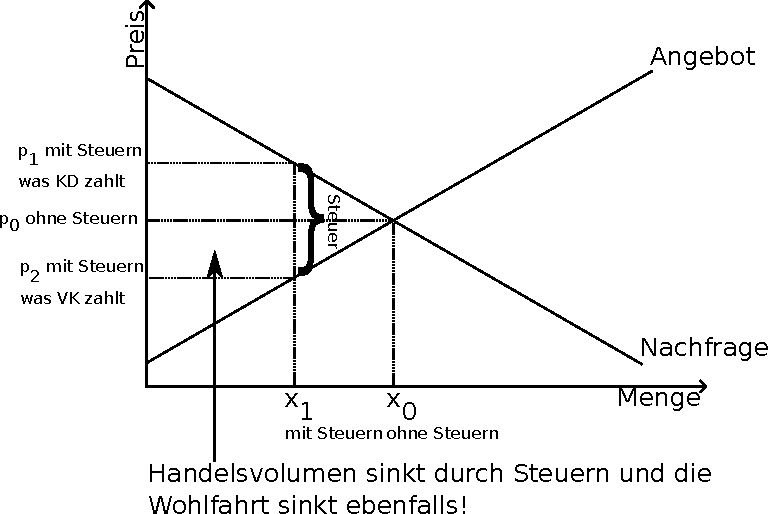
\includegraphics[]{ProdKonsRentemitSteuern.pdf}
     \caption{Die Besteuerung eines Marktes}
     \label{fig:bild}
\end{figure}

Der Code für Beispielbild 1%~/ref{fig:bild}.
..an dieser Stelle würde ich gerne mit \textbackslash ref das Bild referenzieren, leider funktioniert das aktuell noch nicht!

Das erste Bild, \glqq Die Besteuerung eines Marktes\grqq, wurde mit dem Parameter \glqq h!\grqq\ aufgerufen. Für \LaTeX{}\ heißt dass, das Bild an Ort und stelle abzulegen.%~\ref{} i need to include all other listings in floats

\begin{lstlisting}[float=htpb,caption=Einbindung einer Grafik so nah wie möglich am Text,label=lst:float_h]
  \begin{figure}[h!]
    \centering
       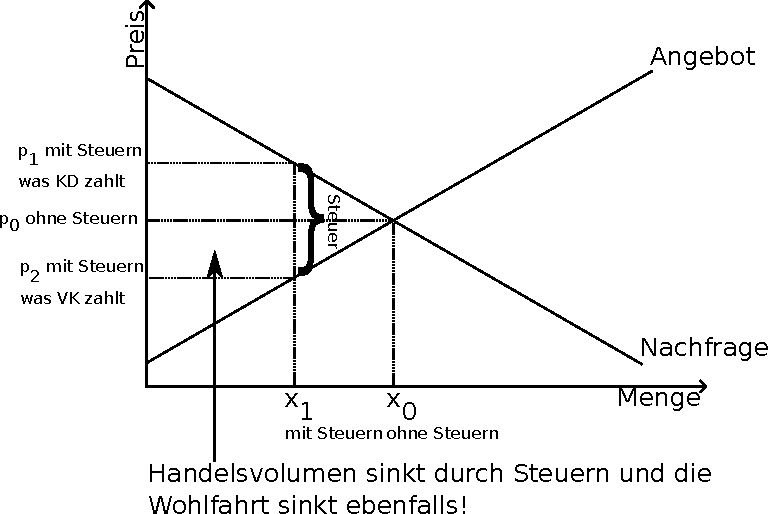
\includegraphics[]{ProdKonsRentemitSteuern.pdf}
    \caption{Die Besteuerung eines Marktes}
    \label{fig:bild}
  \end{figure}
\end{lstlisting}

Eine zweite Grafik zum rumschieben, dieses mal hat \LaTeX{}\ mehr Freiheiten, durch \glqq htbp\grqq.

\begin{figure}[htbp]
  \centering
     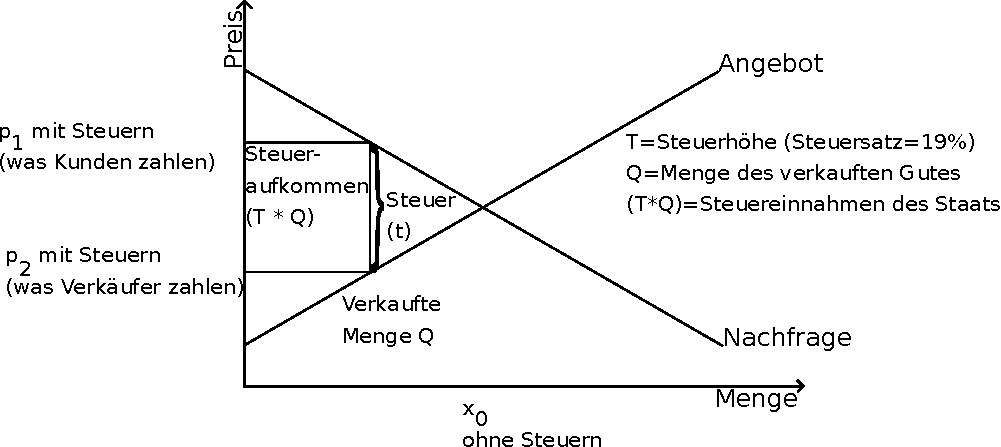
\includegraphics[width=1\linewidth]{PMSteuer.pdf}
  \caption{Steueraufkommen}
  \label{fig:bild2}
\end{figure}

Hier schreibe ich noch mal etwas Text hin, der keinen Sinn ergibt, wenigstens zwangsläufig, immerhin soll \gls{latex} rund um meine beiden Beispielbilder etwas Text zu verarbeiten haben, damit der Leser/Anwender es später selbst etwas einfacher hat, sich das Konzept vor Augen zu führen. Kommentiert einfach etwas Text raus, ändert die Größe der Grafiken oder die angegebenen Parameter und ihr solltet ein Bild davon bekommen, was \LaTeX{}\ sich bei der Sache denkt.

Zusätzlich erhält dieser Block einen neuen Absatz. Das Thema Bienensterben ist ein ernstes Thema auf welches man an dieser Stelle aufmerksam machen kann, da sie sehr wichtig für das Ökosystem unseres Planeten sind.

\begin{lstlisting}[float=htpb,caption=Automatische Einbindung einer Grafik,label=lst:float_htbp]
  \begin{figure}[htbp]
    \centering
       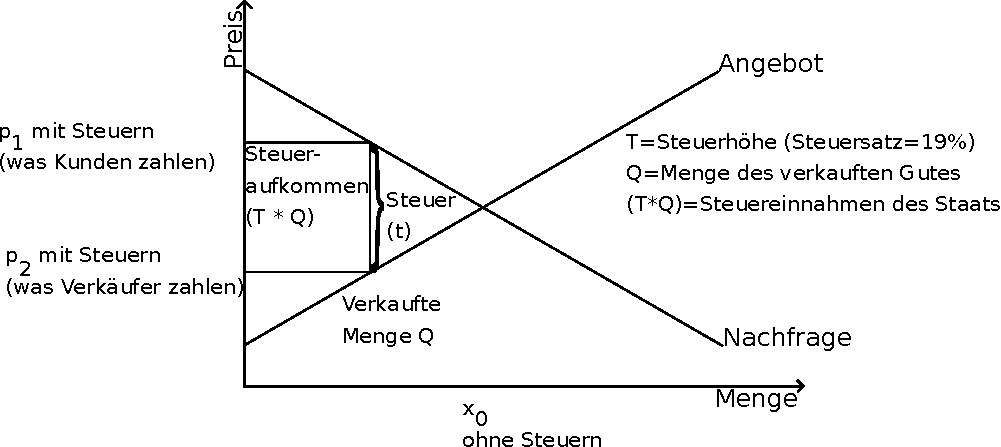
\includegraphics[width=1\linewidth]{PMSteuer.pdf}
    \caption{Steueraufkommen}
    \label{fig:bild2}
  \end{figure}
\end{lstlisting}
%}}}
\subsection{Grafiken mit TikZ}%{{{
\label{sec:tikzgraph}
\LaTeX{} bietet eine eigene \emph{Vektorzeichenumgebung} an: \glqq TikZ\grqq! Selbst habe ich es noch nicht verwendet, allerdings passt die Art sehr gut in das Gesamtdokument. Darüber hinaus folgt die Syntax einer relativ einfachen Logik, was also durchaus bei kleineren Grafiken Zeit sparen kann.

\begin{tikzpicture}
  [level 1/.style={sibling distance=35mm,
    level distance=20mm},
    level 2/.style={sibling distance=15mm,
    level distance=10mm}]
  \node {Planzen}
    child {node {Blumen}
    child {node {Rosen}}
    child {node {Nelken}}
    child {node {\ldots}}
  }
    child {node {Bäume}
    child {node {Tanne}}
    child {node {Eiche}}
  };
\end{tikzpicture}

Folgendes Beispiel stammt von Christine Römer\footcite{dtk17.1:roemer:tikz} und wurde in \glqq Die \TeX{}nische Komödie\grqq\ veröffentlicht. Die Zeitschrift wird von \glspl{dante} herausgegebenen.
%}}}
\subsection{Fußnoten}%{{{
\label{sec:footn}
Fußnoten werden über den Befehl \textbackslash footnote gesetzt und automatisch im Footer fortlaufend Nummeriert aufgeführt.\footnote{\href{https://de.wikibooks.org/wiki/LaTeX-W\%C3\%B6rterbuch:_footnote}{Mehr auf Wikibooks}}
\begin{lstlisting}[float=htpb,caption=Das setzen von Fußnoten mit \protect\LaTeX{},label=lst:footnotes]
Fußnoten werden über den Befehl \footnote{Meine erste Fußnote} gesetzt und automatisch im Footer fortlaufend Nummeriert aufgeführt.\footnote{\href{https://de.wikibooks.org/wiki/LaTeX-W\%C3\%B6rterbuch:_footnote}{Mehr auf Wikibooks}}
\end{lstlisting}
%}}}
\subsection{Code}%{{{
\label{sec:code}
Code wird am Besten, genau wie eine Grafik (siehe Kapitel~\ref{sec:graphics}), in einer eigenen Umgebung eingefügt. Erstens kümmert sicht \gls{latex} nun selbstständig um die Platzierung, zweitens können wir dem \glqq Float\grqq\ ein Label verpassen, dass wir dann referenzieren können.

\lstset{language=Ruby}
\begin{lstlisting}[float=htpb,caption=Beispielcode,label=bspcode]
#!/usr/bin/env ruby

listofstrings = ARGV
puts listofstrings.sort.uniq
\end{lstlisting}

Der Code hierfür:
\begin{lstlisting}[float=htpb,caption=Darstellung eines beliebigen Codes in der Sprache ruby,label=lst:ruby]
\lstset{language=Ruby}
\textbackslash begin{lstlisting}[float=htpb,caption=Beispielcode,label=bspcode]
#!/usr/bin/env ruby

listofstrings = ARGV
puts listofstrings.sort.uniq
\textbackslash end{lstlisting}
\end{lstlisting}
Es ist möglich, die dargestellte Sprache anzupassen, das zeigt \textbackslash\{language=Ruby\}. Für das Beispiel musste ich aber die begin/end-Umgebung aufbrechen, da ansonsten der Compiler durcheinander kommt.

Sollte man diese Funktion gar nicht gebrauchen, kann man die letzten Zeilen in der Präambel dafür kommentieren, damit die Pakete nicht zwingend geladen werden müssen. Das sollte die Performance steigern und mögliche Kompatibilitätsschwierigkeiten, sofern vorhanden, zuvorkommen.
%}}}
\subsection{Zitieren}%{{{
Zitation scheint mit eines der heikeligsten Angelegenheiten in einer Thesis zu sein. Muss es aber gar nicht. Denn hier kommt \hologo{BibTeX}.

Dieses Sektion wurde außerdem mit Hilfe der üblichen Internetadressen (vorwiegend \href{https://tex.stackexchange.com/}{TeX - LaTeX Stack Exchange}), aber auch einem Blick ins Handbuch von biblatex \footcite{lehman_biblatex_2017}, vorzugsweise in der englischen Originalfassung \footcite{kime_biblatex_2019}, da das Paket ständig überarbeitet wird und somit neue Optionen dazukommen, oder bekannte Optionen ersetzt werden, geschrieben.

Es sei zu erwähnen, das biber\footcite[][]{kime_biber_2019} ebenfalls ein eigenes Handbuch hat, dass weiterhelfen kann!

\begin{lstlisting}[float=htpb,caption=Das Setzen von Zitations \protect\LaTeX{},label=lst:cites]
Es sei zu erwähnen, das biber\footcite[][]{kime_biber_2019} ebenfalls ein eigenes Handbuch hat, dass weiterhelfen kann!
\end{lstlisting}
Relevanter Code:
\lstinputlisting[firstline=116,lastline=137,float=htpb,caption=Relevanter Code für biblatex,label=lst:our-bib]{meta/preambel.tex}

In Tabelle ~\ref{tab:bib-style} will ich eine kleine Übersicht über die verfügbaren Stile gestalten. Wir benötigen den \gls{apa}-Stil.

\begin{table}[htbp]
\centering
\resizebox{\textwidth}{!}{%
\begin{tabular}{l|l|l|}
\hline
\multicolumn{1}{|l|}{\textbf{Option}} & \textbf{Wert} & \textbf{\begin{tabular}[c]{@{}l@{}}nennenswerter \\ Effekt\end{tabular}} \\ \hline
\multicolumn{1}{|l|}{autocite} & footnote & Setzt eine Fußnote \\ \hline
 & cite & setzt den Verweis direkt im Text \\ \cline{2-3}
 & parencite & setzt den Verweis im Text in Klammern \\ \hline
\multicolumn{1}{|l|}{style} & numeric & \begin{tabular}[c]{@{}l@{}}Literatur wird numerisch im Verzeichnis\\ aufgeführt\end{tabular} \\ \hline
 & numeric-comp & \begin{tabular}[c]{@{}l@{}}Wie oben, aber mehrerer aufeinanderfolgende\\ Werke werden zusammengefasst\end{tabular} \\ \cline{2-3}
 & alphabetic & \begin{tabular}[c]{@{}l@{}}Erstellt ein Kürzel des Autors und hängt eine\\ fortlaufende Ziffer dran (numeric Verhalten)\end{tabular} \\ \cline{2-3} 
 & authoryear & Sortiert nach Autor und Jahr \\ \cline{2-3}
 & authoryear-comp & siehe oben \\ \cline{2-3}
 & authoryear-ibid & setzt ein ebenda, bzw. ebd. \\ \cline{2-3}
 & authoryear-icomp & vereint -comp und -ibid \\ \cline{2-3}
 & authortitle & Sortiert nach Autor und Jahr \\ \cline{2-3}
 & authortitle-comp & siehe oben \\ \cline{2-3}
 & authortitle-ibid &  \\ \cline{2-3}
 & authortitle-icomp &  \\ \cline{2-3}
 & authortite-terse & \begin{tabular}[c]{@{}l@{}}Lässt den Titel aus, wenn der Author nur ein\\ Werk in unserem Literaturverzeichnis hat\end{tabular} \\ \cline{2-3}
 & authortitle-tcomp & Vereint -comp und -terse \\ \cline{2-3}
 & authortitle-ticomp & -comp, -ibid, -terse \\ \cline{2-3}
 & apa & ziemliche vollständiger \gls{apa} Stil der 6ten Edition \\ \cline{2-3}
\end{tabular}%
}
\caption{Einige Optionen zu verwendbaren Zitationsstilen}
\label{tab:bib-style}
\end{table}

Die Idee hinter \hologo{BibTeX}\ ist, dass man die Werke einmalig in einer Datenbank erfasst und von dort aus mit einem zugewiesenem \glqq citekey\grqq\ referenziert. Die Erstellung und Verwaltung einer Datenbank ist z.B. über \href{https://www.zotero.org/}{Zotero}\ (Quelloffen), \href{https://www.jabref.org/}{JabRef}\ (Quelloffen) und \href{https://www.citavi.com/}{Citavi}\ (Closed Source) möglich. Da es sich aber, wie bei \LaTeX{}\ üblich um eine einfache Textdatei handelt, kann man die Datenbank auch selbst
schreiben. Das ist vor allem bei kürzeren Werken eine Alternative, wo man nur mit wenigen Quellen arbeiten muss.
Mir hat bei der Verwendung zotero gut geholfen. Auch hier empfiehlt sich ein Einarbeiten in das Programm, da es doch sehr viele Möglichkeiten zur Verwaltung der genutzten Literatur bietet.

Das hier ist ein Testzitat für einen Aufsatz in einem Sammelwerk\footcite[][]{billen_kundenbindung_2005}, damit wir den genutzten Stil austesten können.

Es ist ebenfalls möglich, ein Zitat im Text in Klammern zu setzen, so wie es z.B. in der Informatik üblicher ist. Dafür ein weiteres Beispielzitat: Lamport \parencite[Siehe][]{lamport_latex_1994} hat das von Don Knuth \parencite[Siehe][]{knuth_tex_1979} erstellte \TeX{} überarbeitet und \LaTeX{}\ programmiert. \LaTeX{}\ macht den Umgang mit \TeX{}\ deutlich einfacher! Vielen Dank an dieser Stelle an Don E. Knuth und L. Lamport, Richard Stallman, Markus Kohm, sowie allen CTAN-Maintainern und Contributern und vielen mehr! Dank euch ist meine Arbeit hier möglich!

Abschließend ein Verweis direkt im Text auf Richard Stallman, \cite[siehe ][S. 6 -- 18]{dibona_open_1999}.
%}}}
\subsection{Querverweise}%{{{
\label{sec:refs}
Leider scheinen Querverweise auf Grafiken gerade nicht zu funktionieren, ein Verweis auf Kapitel~\ref{sec:graphics} funktioniert aber. Ich werde mich der Sache zu einem anderen Zeitpunkt noch mal widmen.

Mal schauen ob ein Querverweis zu ~\ref{bspcode} funktionieren. Tabelle~\ref{tab:textformat} funktioniert auch.
%}}}
\subsection{Verzeichnisse}%{{{
\label{sec:catalogs}
\gls{latex} macht es verhältnismäßig einfach, Verzeichnisse zu führen, das ist aber auch einer der Gründe, warum wir den \gls{latex}-\gls{compiler} mehrfach laufen lassen müssen (vgl. Listing~\ref{lst:arara-rules}). \gls{latex} erstellt bei den ersten Durchläufen Hilfsdateien, die dann ferner von anderen Tools aufgegriffen und verarbeitet werden. Bei dem nächsten Compileraufruf weiß \gls{latex} dann genau, wo es welche Verweise setzen muss. Dies geschieht nicht immer Fehlerfrei, deswegen ist ein prüfender Blick vor der Abgabe dennoch zu empfehlen.

\lstinputlisting[firstline=4,lastline=14,float=htpb,caption=arara regeln,label=lst:arara-rules]{main.tex}
Anbei sind folgende hier im Code verwendete erklärt.
%}}}
\subsubsection{Inhaltsverzeichnis}%{{{
\label{sec:toc}
Ein Inhaltsverzeichnis wird einfach über \textbackslash tableofcontents eingefügt\footcite[Vgl. ][S. 7ff]{ochsner_textverarbeitungssystem_2015}.

\lstinputlisting[firstline=52,lastline=54,float=htpb,caption=Unser Inhaltsverzeichnis,label=lst:ourtoc]{main.tex}

Wie wir anhand von Listing~\ref{lst:ourtoc} in Zeile 2 sehen können, haben wir hier schon die Möglichkeit genutzt, die Tiefe des Inhaltsverzeichnisses anzupassen. Für weitere Optionen ist weiterführende Literatur empfehlenswert, mir hat das Werk von Schlosser gut weitergeholfen.\footcite[Vgl. ][S. 207ff.]{schlosser_wissenschaftliche_2014}
%}}}
\subsubsection{Abbildungsverzeichnis}%{{{
\label{sec:lof}
Abbildungen werden über \textbackslash listoffigures aufgelistet. Damit eine Abbildung im Verzeichnis aufgenommen wird, muss die \textbackslash begin\{figure\}\ldots end\{figure\}-Umgebung genutzt werden. Durch die darin genutzte Option \textbackslash caption\{ \ldots \} hat das Kind auch direkt einen Namen.
%}}}
\subsubsection{Abkürzungsverzeichnis}%{{{
\label{sec:acros}
Das Abkürzungsverzeichnis wird über das Paket glossaries erstellt. Die Definition der Abkürzungen geschieht über meta/acro.tex.

Der Code für glossaries wird einmalig für mehrere Zwecke verwendet, hier allerdings einmalig eingeblendet.

\lstinputlisting[firstline=140,lastline=149,float=htpb,caption=Relavanter Code für das Abkürzungsverzeichnis,label=lst:our-acros]{meta/preambel.tex}
%}}}
\subsubsection{Glossar}%{{{
\label{sec:glossaries}
Ein Glossar soll dem Leser Fachbegriffe näher bringen. In einem gesonderten Verzeichnis im Anhang werden die definierten Begriffe dann aufgelistet.

\lstinputlisting[firstline=151,lastline=156,float=htpb,caption=Relevanter Code für unser Glossar,label=lst:our-glo]{meta/preambel.tex}

Die Glossareinträge sind in meta/gls.tex definiert.
%}}}
\subsubsection{Index}%{{{
\label{sec:xindy}
Schreiben sie von \index{Alpha}Alpha bis \index{Omega}Omega.

\begin{lstlisting}[float=htpb,caption=Das setzen von Indextoken mit \protect\LaTeX{},label=lst:indextoken]
Schreiben sie von \index{Alpha}Alpha bis \index{Omega}Omega.
\end{lstlisting}

Mit einem Index kann man Schlagworte und Themengruppen zusammenfassen und dem Leser helfen, diese im Dokument zu finden.

\lstinputlisting[firstline=156,lastline=161,float=htpb,caption=Relevanter Code für unseren Index,label=lst:our-idx]{meta/preambel.tex}%}}}
%}}}

% !TEX root = ../main.tex
\newpage
\section{Spaß mit LaTeX}
\subsection{Mathe}
\label{sec:}

Expand $(a+b)^n$:
\newcount\mycntr

  \begin{center}
    \mycntr=0
    \loop\advance\mycntr by 1
    \ifnum\mycntr<20
      $(a\hskip\mycntr pt +\hskip\mycntr pt b)^n$\\
    \repeat
  \end{center}

If~~$\displaystyle\lim_{x\rightarrow8}\frac{1}{x{-}8}=\infty$
~~then~~$\displaystyle\lim_{x\rightarrow5}\frac{1}{x{-}5}=\rotatebox{90}{5}$

\subsection{TikZ}
\label{sec:tikz}
\resizebox{\textwidth}{!}{%
\tikz{
    \draw(-10,-10)rectangle+(20,20);
    \foreach\x/\y in{
        -1/ 1,  0/ 1,  1/ 1,
        -1/ 0,  0/ 0,  1/ 0,
        -1/-1,  0/-1,  1/-1,
          -.5/ .5, .5/ .5,
          -.5/-.5, .5/-.5
    }{
        \begin{scope}
            \tikzset{shift={(\x*6.6,\y*6.6)},xscale=(-1)^(\x+\y)}
            \pgflowlevelsynccm
            \foreach\j in{1,...,15}{
                \draw[line width=6mm,
                    dash pattern={on13.408ptoff13.408pt},
                    dash phase=\j*13.408pt]
                    circle(3);
                \draw[line width=6mm,white,
                    dash pattern={on13.408ptoff13.408pt},
                    dash phase=(\j+1)*13.408pt]
                    circle(3);
                \foreach\i in{1,...,20}{
                    \tikzset{rotate=\i*18+\j*9}
                    \fill[yellow!80!black]
                        (3,0)ellipse[x radius=3mm,y radius=1.5mm];
                    \tikzset{rotate=9}
                    \fill[blue]
                        (3,0)ellipse[x radius=3mm,y radius=1.5mm];
                }
                \tikzset{scale=.81818}
                \pgflowlevelsynccm
            }
        \end{scope}
    }
}
}

%%% HSD-LaTeX-Template (c) by Tim Biermann
%%%
%%% HSD-LaTeX-Template is licensed under a
%%% Creative Commons Attribution-ShareAlike 4.0 International License.
%%%
%%% You should have received a copy of the license along with this
%%% work. If not, see <http://creativecommons.org/licenses/by-sa/4.0/>.

% !TEX root = ../../main.tex
\newpage
\section{Fazit}
Wie wir sehen, ist \LaTeX{} ganz schön toll. Ich jedenfalls würde es meinen Freunden und meiner Familie empfehlen!

Abschließend ist euch allen viel Erfolg für die Thesis zu wünschen!


\clearpage % force latex to place anything not yet placed before proceeding
\pagenumbering{Roman} % change back to Roman page numbering style
\setcounter{page}{8}  % change the number accordingly

%%% Glossaries
\newpage
\phantomsection % fixes wrong page numbering
\printglossary[type=main]

%%% print index
\newpage
\phantomsection % fixes wrong page numbering
\addcontentsline{toc}{section}{Index}
\printindex

%%% print bibliography
\newpage
\renewcommand{\refname}{Literaturverzeichnis} % rename "Literatur" to "Literaturverzeichnis"
\phantomsection % fixes wrong page numbering

%\printbibliography % print the bibliography as a whole

%%% you can also split your bibliography by type like this
\printbibliography[keyword=main] % print all cites used throughout our work
\printbibliography[keyword=ctan,heading=subbibliography,title={CTAN Pakete}] % additionally, cite all packages used

%%% appendix
\newpage
\phantomsection % fixes wrong page numbering
\addcontentsline{toc}{section}{Appendix}
\appendix

%%% Attachment A

\includepdf[scale=.7,pages=1, offset=0 -3cm,pagecommand=\section{Prüfungsordnung Wirtschaft}]{content/attachments/po_wiwi.pdf}
%%% this effectively works around the sectioning issue of a multi page pdf

\includepdf[scale=.7,pages=2-7, offset=0 -3cm]{content/attachments/po_wiwi.pdf}

%%% Attachment B
% !TEX root = ../../main.tex
% Kapitel

\section{Tipps zu häufig gemachten Fehlern}

\subsection{Abbildungen, Tabellen, Listings, etc.}
\begin{enumerate}
 \item Die Schriftgröße von Text in Abbildungen muss sich nach der Schriftgröße
 des regulären Textes richten.
 \item Alle Abbildungen, Tabellen, Listings, etc. sind mit einer Beschriftung
 und Nummerierung zu versehen. Im Text muss mit Hilfe der Nummerierung auf
 die jeweilige Abbildung, Tabelle bzw. das Listing, etc. verwiesen und eine
 Erläuterung der Abbildung, Tabelle bzw. des Listings verfasst werden.
\end{enumerate}

\subsection{Text}
\begin{enumerate}
 \item Abkürzungen werden einmalig wie in Abschnitt~\ref{sec:acros} beschrieben eingeführt
 und verwendet.
 \item Fachbegriffe müssen eingeführt und definiert werden. Der Fachbegriff kann
 z. B. einmal \textit{kursiv} gedruckt und danach normal geschrieben werden. Für
 die Definition und Erklärung sollte einschlägige Literatur verwendet werden.
 \item Es muss eine Rechtschreib- und Grammatikprüfung verwendet werden.
 \item Es sollte eine Korrektur durch Dritte durchgeführt werden.
 \item Es muss Groß-/Kleinschreibung im Literaturverzeichnis beachtet werden.
 \item Es müssen Deutsche Anführungsstriche verwendet werden: \glqq \dots\grqq
\end{enumerate}

\subsection{Diverses}
\begin{enumerate}
 \item Wenn es sich bei der Arbeit um einen Angriff dreht, dann muss
 (am Besten am Beginn der Arbeit) die Hackerethik zusammenfassend beschrieben
 und dabei konkret auf den Angriff bezogen werden.
 \item Internetquellen sollen nicht in das Literaturverzeichnis, sondern über
 eine Fußnote unter Angabe der URL und dem letzten Abrufdatum dokumentiert
 werden.
\end{enumerate}


%%% last page
% !TEX root = ../../main.tex
\newpage
\clearpairofpagestyles
%\lehead{
\includegraphics[width=3.8cm]{HSD_logo.pdf}} % this sets the picture way to high
%\lohead{
\includegraphics[width=3.8cm]{HSD_logo.pdf}}
\KOMAoptions{headsepline=0pt}
\pagenumbering{gobble} % no page numbering

\includegraphics[width=5cm]{HSD_logo.pdf}
\section*{Eidesstattliche Versicherung}
\_\_\_\_\_\_\_\_\_\_\_\_\_\_\_\_\_\_\_\_\_\_\_\_ \hspace{1.5cm} \_\_\_\_\_\_\_\_\_\_\_\_\_\_\_\_\_\_\_\_\_\_\_\_ \\
\small{Name, Vorname}\hspace{4.4cm}
\small{Matrikelnummer}
\newline
Hiermit versichere ich an Eides Statt, dass ich die Bachelorarbeit/Masterarbeit (nicht Zutreffendes bitte streichen) mit dem Titel \newline
\_\_\_\_\_\_\_\_\_\_\_\_\_\_\_\_\_\_\_\_\_\_\_\_\_\_\_\_\_\_\_\_\_\_\_\_\_\_\_\_\_\_\_\_\_\_\_\_\_\_\_\_\_\_\_\_\_\_ \\
\_\_\_\_\_\_\_\_\_\_\_\_\_\_\_\_\_\_\_\_\_\_\_\_\_\_\_\_\_\_\_\_\_\_\_\_\_\_\_\_\_\_\_\_\_\_\_\_\_\_\_\_\_\_\_\_\_\_ \\
eigenständig und ohne unzulässige fremde Hilfe verfasst habe. Ich habe keine anderen als die angegebenen Quellen und Hilfsmittel benutzt und die aus fremden Quellen direkt oder indirekt übernommenen Inhalte als solche kenntlich gemacht. Für den Fall, dass die Arbeit zusätzlich auf einem Datenträger eingereicht wird, erkläre ich, dass die schriftliche und die elektronische Form vollständig übereinstimmen. Die Arbeit hat in gleicher oder ähnlicher Form noch in keinem Prüfungsverfahren vorgelegen.
Sie wurde auch nicht veröffentlicht. Ich erkläre mich damit einverstanden, dass die Arbeit mit Hilfe computergestützter Methoden auf Plagiate hin überprüft wird.\newline
\_\_\_\_\_\_\_\_\_\_\_\_\_\_\_\_\_\_\_\_\_\_\_\_ \hspace{1.5cm} \_\_\_\_\_\_\_\_\_\_\_\_\_\_\_\_\_\_\_\_\_\_\_\_ \\
\small{Ort, Datum}\hspace{4.8cm}
\small{Unterschrift}
\newline
\textbf{Belehrung:}\newline
Die vorsätzlich oder auf nur fahrlässig falsche Abgabe einer eidesstattlichen Versicherung ist strafbar:\newline
\newline
\textbf{\S\ 156 StGB - Falsche Versicherung an Eides Statt}\newline
WWer von einer zur Abnahme einer Versicherung an Eides Statt zuständigen Behörde eine solche Versicherung falsch abgibt oder unter Berufung auf eine solche Versicherung falsch aussagt, wird mit Freiheitsstrafe bis zu drei Jahren oder mit Geldstrafe bestraft.\newline
\textbf{\S\ 161 StGB - Fahrlässiger Falscheid; fahrlässige falsche Versicherung an Eides Statt}
(1) Wenn eine der in den \S\S\ 154 bis 156 bezeichneten Handlungen aus Fahrlässigkeit begangen worden ist, so tritt die Freiheitsstrafe bis zu einem Jahr oder Geldstrafe ein.
(2) Straflosigkeit tritt ein, wenn der Täter die falsche Angabe rechtzeitig berichtigt. Die Vorschriften des \S\ 158 Abs. 2 und 3 gelten entsprechend.\newline
\newline
Die vorstehende Belehrung habe ich zur Kenntnis genommen:\newline
\newline
\_\_\_\_\_\_\_\_\_\_\_\_\_\_\_\_\_\_\_\_\_\_\_\_ \hspace{1.5cm} \_\_\_\_\_\_\_\_\_\_\_\_\_\_\_\_\_\_\_\_\_\_\_\_ \\
\small{Ort, Datum}\hspace{4.8cm}
\small{Unterschrift}
 % sworn declaration

\end{document}
